\documentclass[journal]{IEEEtran}
\usepackage{blindtext}
\usepackage{listings} % needed for the inclusion of source code
\usepackage{hyperref} % for hyperlinks - Jared 9/28/17
\usepackage{url} % for hyperlinks - Jared 9/28/17
\usepackage{graphicx}
\usepackage{wrapfig}
\usepackage{array}
\graphicspath{ {images/} }

%Used to display java code
\usepackage{color}
\definecolor{dkgreen}{rgb}{0,0.6,0}
\definecolor{gray}{rgb}{0.5,0.5,0.5}
\definecolor{mauve}{rgb}{0.58,0,0.82}

\lstset{ %
  language=Java,                  % the language of the code
  basicstyle=\footnotesize,       % the size of the fonts that are used for the code
  numbers=left,                   % where to put the line-numbers
  numberstyle=\tiny\color{gray},  % the style that is used for the line-numbers
  stepnumber=0,                   % the step between two line-numbers. If it's 1, each line 
                                  % will be numbered
  numbersep=5pt,                  % how far the line-numbers are from the code
  backgroundcolor=\color{white},  % choose the background color. You must add \usepackage{color}
  showspaces=false,               % show spaces adding particular underscores
  showstringspaces=false,         % underline spaces within strings
  showtabs=false,                 % show tabs within strings adding particular underscores
  frame=,                         % single adds a frame around the code
  rulecolor=\color{black},        % if not set, the frame-color may be changed on line-breaks within not-black text (e.g. commens (green here))
  tabsize=4,                      % sets default tabsize to 2 spaces
  captionpos=b,                   % sets the caption-position to bottom
  breaklines=true,                % sets automatic line breaking
  breakatwhitespace=false,        % sets if automatic breaks should only happen at whitespace
  caption=\lstname,
  %title=\lstname,                 % show the filename of files included with \lstinputlisting;
                                  % also try caption instead of title
  keywordstyle=\color{blue},          % keyword style
  commentstyle=\color{dkgreen},       % comment style
  stringstyle=\color{mauve},         % string literal style
  escapeinside={\%*}{*)},            % if you want to add a comment within your code
  morekeywords={*,...}               % if you want to add more keywords to the set
}
%End of defs for java syntax highlighting

\begin{document}
% Possible Journal to Submit to: Pattern Recognition Letters  - Jared 9/28/1
% Title Area
% paper title
% can use linebreaks \\ within to get better formatting as desired
\title{Supervised Machine Learning Using Object-Oriented Programming Principles}
% - Changed title to be more specific - Jared 8/31/17 
\author{Merl~Creps Jr,~\IEEEmembership{Member,~IEEE}\\
Jared ~Oluoch, Member, ~IEEE}% The paper headers

\markboth{Journal of \LaTeX\ Class Files,~Vol.~6, No.~1, January~2007}%
{Shell \MakeLowercase{\textit{et al.}}: Bare Demo of IEEEtran.cls for Journals}

\maketitle


\begin{abstract}
%\boldmath
%Needs to be re-written wneh paper is complete - jo 9/28/17
This paper presents a case study for supervised machine learning using object-oriented programming principles. For this purpose, objects are used to represent various complex data structures within the machine learning algorithm. 
\end{abstract}


\begin{IEEEkeywords}
Artificial Intelligence, Artificial neural networks, Cognitive Complexity, Design Principals, Design Methodology, Machine Learning, Object oriented programming, Software Engineering, Supervised Learning
\end{IEEEkeywords}

% For peer review papers, you can put extra information on the cover
% page as needed:
% \ifCLASSOPTIONpeerreview
% \begin{center} \bfseries EDICS Category: 3-BBND \end{center}
% \fi
%
% For peerreview papers, this IEEEtran command inserts a page break and
% creates the second title. It will be ignored for other modes.
\IEEEpeerreviewmaketitle


\section{Introduction}
Object-oriented programming (OOP) is a paradigm that combines data and instruction sets for processing data into objects that are used within an application. It provides crucial concepts that assist with modelling complicated real world systems into reusable, manageable, and maintainable software solutions.  In addition, it provides a more seamless transition between the different phases of the software life-cycle.


%\subsection{Abbreviations and Acronyms} - We do not need this section. - Jared 8/31/17
%Object orientated programming OOP, Unified Modeling Language UML

%Object-oreintated programming introduction
%\section{Object Orientated Programming} - Combine this section with the intro - Jared 8/31/17
OOP refers %to a programming paradigm  -jo 9/28/17
models entities based on objects, classes, polymorphism, inheritance and abstraction.  These objects are organized into classes, which allow individual objects to be group together. Modern programming languages such as Java, C/C++, Objective-C, Ruby, Grails, and PHP, are object-oriented. 


%Object-oriented programming  - Jared 9/26/17
OOP simplifies and organize software applications to allow software engineers to focus on the specific application context. Individual objects can be modified without affecting other aspects of the application. As software applications have increased in size and complexity, OOP has improved the development cycles for large, complex applications
% ADDED - JARED 9/26/17
and made them more manageable.


%define the key concepts of OOP
\subsection{Objects}
Objects are the self-contained, fundamental building blocks in OOP with a great emphasis placed on the applications design and functionality.  An object contains all the necessary attributes and methods that make the objects useful when designing solutions to complex problems.  An object's attributes are all the pertinent information that describe the functionality of the object.  


\subsection{Classes}
Classes are a fundamental part of object-orientated programming and are used to describe one or multiple objects.  Classes provided concrete implementation for instantiating specific objects within the application.  An object is derived from a single class, but can instantiate multiple objects during the application.  While classes are at the core of OOP, classes must be instantiated as objects in order to be used by any application. 

Classes allow for a layer of encapsulation, which isolates variables and methods for specific instantiated objects.  This encapsulation protects each class from modifications from other classes or by the software engineer in other areas of the application.  By using classes, software engineers can create well-organized code which can easily be maintained. 
%Added - Jared 9/26/17
Listing 1 illustrates a source code for a neural network exception class.

%display sample class
\lstinputlisting[language=Java]{SourceCode/NeuralNetException.java}


\subsection{Inheritance}
Inheritance %is specific to %object-oriented programming, - jo 9/28/17
%OOP, and - jo 9/28/17
is a concept by which an object acquires all the attributes and methods of the base or parent object.  An inherited class is referred to as a subclass of its parent or super class. The subclass does not need to have a formal definition of it's attributes or methods that are inherited from the parent class.  Inheritance %is a mechanism which  - jo 9/28/17
promotes code reuse and to allow the code to be extended through the original software using public classes, abstract classes, and interfaces. 
% Added - Jared 9/26/17
Listing 2 illustrates an inheritance class.

\newpage
\lstinputlisting[language=Java]{SourceCode/inheritance_example.java}


\subsection{Polymorphism}
Polymorphism is a concept in %object-orientated programming 
OOP where the software engineer can assign different meanings or usages based upon 
%the context or meaning.  Jared 9/26/17
a given context.
Polymorphism provides the mechanics to have variables, function or objects to have more than one form.  Polymorphism takes several forms; variables, functions, and machine leaning.

\begin{itemize}
    \item Variables may take on the form of an integer in one context but transform into a string in another context.  Take userId, this may be an integer or string depending on the context.

    \item Function or methods can have the same name but have a different set of formal parameters and may even return a different data type based upon the context.

    \item Machine learning language, a data type of ``any", such that when specified for a list, a list containing any data types can be processed by a function. If a function simply determines the length of a list, it doesn't matter what data types are in the list
\end{itemize}


\lstinputlisting[language=Java]{SourceCode/polymorphism_example.java}

\subsection{Abstraction}
Abstraction is one of the fundamental concepts of 
%object-oriented programming - Jared 9/26/17
OOP focusing on what, not how.  Abstraction allows complex extraneous details to be suppressed by creating a level of complexity that the software engineer will interact with the system.  Abstraction lets the software engineer focus on the application, not the ancillary details that can be %abstracted or - Jared 9/26/17.
generalized into reusable components.

% Added - Jared 8/31/17 : You need to add a paragraph here that summarizes what this paper accomplishes by using OOP and machine learning. Eaxmple...

% Section added 5-Sept-2017 MJC
%In conclusion, this article will attempt to show that an objectified or OOP approach will lead to a more sustainable machine learning algorithm while implementing a simpler application interface.  The OOP implementation will provide a more efficiency and accuracy prediction model. -Jared 9/26/17
This paper utilizes an OOP approach to design a machine learning algorithm that provides an efficient and accurate prediction model. % Jared - 9/26/17

The rest of this paper is organized as follows. Section II discusses literature that closely relates to our work. Section III describes the artificial neural network developed in this paper. Section IV concludes the paper. % Jared 9/26/17.



\section{Literature Review}
% Jared - 8/31/17
%We need a section here that reviews existing literature. So read relevant papers and summarize what they say about OOP, machine learning, and what you want to accomplish
%Most of the existing literature currently depicts the approach, algorithm, correlates the training input size to the actual input size or the collection methods used to compute Cancer Predictions and Prognosis. - Jared 9/26/17
Object-oriented approach to machine learning is not a new phenomenon. Real world objects are represented in machine learning using idealization and abstraction \cite{tuncc2015semantics}.
Abdrabou and Salem \cite{abdrabou2010breast} designed two object-oriented frameworks for cancer diagnosis. The framework maps all concepts onto classes and interfaces. The framework includes Java classes and a number of XML files. The framework is then organized around tasks and methods. 
In their work, \cite{tosun2009object} use objects to represent tissue components in colon biopsy images. Results of their work demonstrate a 94.89 \% accuracy.
In their study, \cite{zhao2016object} applied an object-oriented regression methodology to analyze High Dimension Omics Data (HDOD) to predict prognonis outcome.

Machine learning employs statistical techniques to learn from past examples in order to predict patterns from large data sets \cite{cruz2006applications}.
These techniques correlate the training input size to the actual input size to compute cancer predictions and prognosis \cite{bartsch2016use}. 
Zhang et al \cite{zhang2017radiomic} utilized radiomics-based prediction of local failure and distant failure in advanced nasopharyngeal carcinoma (NPC). 
Yu and Sun \cite{yu2017sparse} propose a sparse coding algorithm that maps the input feature to a sparse representation. Results of their work demonstrate a more accurate classification than existing solutions.
Moorthy et al., \cite{moorthy2017classification} harvested carcinogenic and mutagenic information of 1481 chemically diverse molecules as their classification models. They correctly classified more than 70 per cent  of compounds in the test set.

Imbus et al., \cite{imbus2017machine} used machine learning and fuzzy-c-means clustering to identify multigland disease in primary hyperparathyroidism among a large data set of patients. They used a boosted tree classifier that had a 94.1 \%  accuracy, 94.1 \% sensitivity, 83.8 \% specificity, and 94.1 \% positive predictive value.
In their study, \cite{kawata2017impact} investigated the impacts of machine learning and Artificial Neural Networks (ANN) for tumor detection of lung cancer. Their finding demonstrated that the framework can be used to identify tumor regions in cancer patients.
In their work, \cite{maniruzzaman2017comparative} adapted a Gaussian process technique to evaluate the accuracy, specificity, sensitivity, positive predictive value, negative predictive value of diabetes.

Jianfu et al., \cite{xia2017ultrasound} used an ultrasound-based machine learning approach to differentiate between benign and malignant thyroid nodules. Results of the study achieved 78.89 \% sensitivity and 94.55 \% specificity.
For machine learning to produce meaningful results, the techniques must be used appropriately \cite{sattlecker2014current}.
Several scholars discuss the collections methods and treatments of the specimens after collection but never the concrete implementation of the algorithm used to make any predictions. 
%(i.e. Use of Artificial Intelligence and Machine Learning Algorithms with Gene Expression Profiling to Predict Recurrent Non-muscle Invasive Urothelial Carcinoma of the Bladder).  
%Another article (i.e Applications of Machine Learning in Cancer Prediction and Prognosis
%) 
%In their work, \cite{} attempted to correlate the training size to the input size and whether the data was over trained by researching various articles on scholar Google and science digest.  
Various learning algorithms such as Decision Trees (DT), Support Vector Machine (SVM), SOM (self organized maps) unsupervised k-maps %(Kohonen 1982), 
, and Naive Bayes have been used in respective prediction, survivability and recurrence models.
%Lastly Computers in Biology and Medicine, 
Existing literature compare a wide variety of algorithms using back-propagation to compute performance indicators.  While the literature  discuss and describe the algorithms, concrete implementations of each of the algorithms is missing. 

Our work differ from existing literature in that we demonstrate the concrete implementation of the Forward feed Neural Network with back-propagation can be successfully designed and rapidly changed to handle a wide variety of ANN algorithms.  We demonstrate that Object-oriented design can and will be successful in ANNs.


\section{Artificial Neural Network}
An Artificial Neural Network (ANN) is a system of interconnected neurons inspired by biological neural systems, such as the human neurological system.  Each ANN is made up of weighted interconnected neurons at each layer that collectively make up the entire neural network.  The neural network was intended to work like the human brain where each neuron represents states, usually a value between 0 and 1.  The neurons and connections act together usually with weights to assist with the learning rate to derive the function.  Neural networks have three layers:% and are as follows - jo 9/28/17
input layer, hidden layer and output layer. 

%Forward Feed - Repeated matrix multiplications interwoven with activation function. 
Machine learning is a sub-discipline of Artificial Intelligence in computer science which allows a computer to learn using input signals or advanced mathematical concepts to provide accurate prediction models.  Machine learning in reality allows a computer to learn without being programmed to provide predictive analytics.  These analytics provide valuable data to data scientists who use them to provided repeated results over and over again.  Machine learning is divided into two categories: supervised or unsupervised.

\begin{itemize}
    \item \textit{Supervised learning} is accomplished using a set of known inputs or training data.  The training data is used to effectively derive the algorithm or function.  Once the algorithm is sufficiently trained, the unknown data set may be examined using the function to accurately predict the desired outcome.  The outcome labels can be analyzed for precision and accuracy because the input data was known. 
    \item \textit{Unsupervised learning} is accomplished by inferring the function or algorithm for an unknown input data set.  In this type of learning both the data inputs and outputs are unknown and the function must determine the correct response.  Unsupervised learning algorithms are solving complex problems with just the input data.
\end{itemize}

\subsection{Multilayer Perceptron}
A multilayer perceptron is a forward feed network, meaning the signal flows in a single direction from the input layer to the output layer until the network is trained.  A MLP consists of a minimum of three layers of connected, neurons which use a non-linear activation function to train the network.  Multilayer perceptron neural networks are generally used to solve problems that involve pattern classification, image recognition, and prediction computations.

\begin{itemize}
    \item \textit{Input layer} is the first layer in the neural network and is the layer that represents the input data set.  The input layer is a passive layer as this layer does not modify any data but rather passes the data onto the hidden layer while consider the weights on each neuron's synopsis.  In a forward feed network, the value or signal sent to each hidden node is the summation of all the connections multiplied by the randomized weights placed on each of those connections.
    \item \textit{Hidden layer} is the layer where the activation function is applied and computes the output.  The hidden layer is an active layer, meaning the neurons modify the signal sent to them from the input streams, and then passes the modified signal to the output layer.
    \item \textit{Output Layer} is the threshold that provides an indicator as to whether the output is present or absent in the input data.  The output layer results are used to compute the error, which is in-turn back-propagated to each input connection.
    
\end{itemize}

\begin{figure}[h]
 \centering
 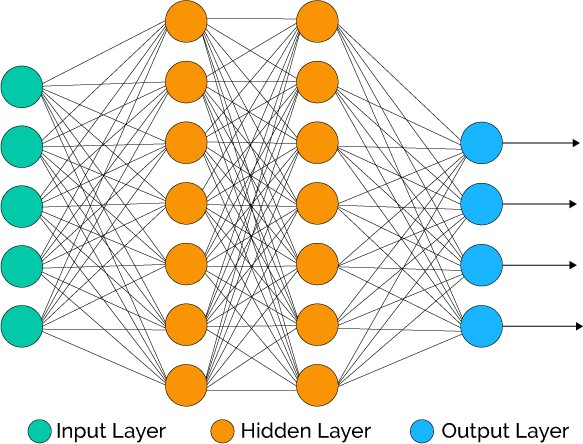
\includegraphics[width=7cm]{network}
 \caption{Deep Artificial Neural Network}
\end{figure}
% jo - 9/28/17
Figure 1 illustrates a deep Artificial Neural Network.
\subsection{Neuron}
The biological neural system is the corner-stone of the artificial neural network since each neuron is mirrored after the biological neuron.  Each neural system contains billions of inter-connected neurons which form the foundation of today's neural networks.  Each neuron in the neural network has the same basic construct.

\begin{figure}[h] %[h] = place here
 \centering
 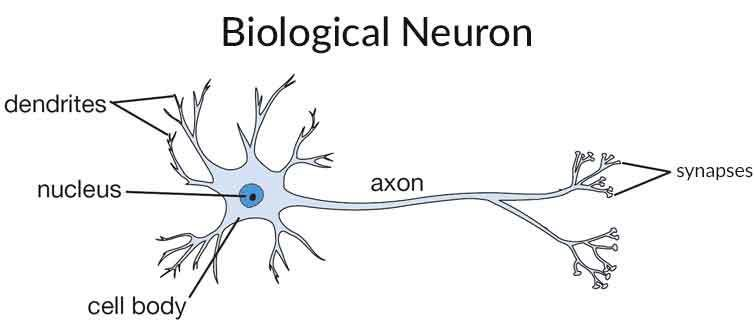
\includegraphics[width=7cm]{neuron}
 \caption{Neuron}
\end{figure}

\subsection{Classifier}
Classifiers are the concrete implementation of mathematical models, functions or algorithms in supervised neural networks to map the inputs into categories.  The classifiers are used in conjunction with training data which is used to train the network for precise and accurate observation as to whether the output data is present or absent in the set of mapped input. 

%Added on 27-Sept-2017 MJC
Classifiers can be separated into two distinct categories, linear and non-linear.  Linear classifier can be thought of as data which can be separated by a single plane.  An example is positive and negatives numbers, a single plane can be drawn between the points which separates them into two distinct groups, positive and negative values.  A non-linear classifier cannot simply separate the data points by a single plane but instead must use multiple plane to organize and group the data.  The rest of the research described in this paper focuses on non-linear classifiers.  Figure 2 and 3 represent linear and non-linear classifiers respectively.

\begin{figure}[h]
\begin{minipage}{.22\textwidth}
  \centering
  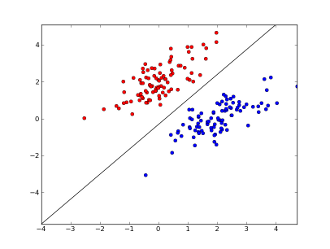
\includegraphics[width=4cm]{linear}
  \caption{Linear}
\end{minipage}%
\begin{minipage}{.22\textwidth}
  \centering
  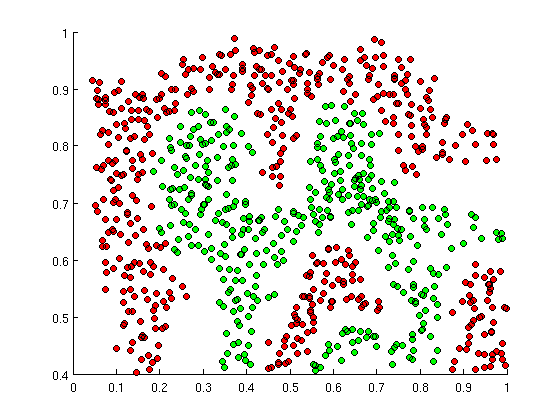
\includegraphics[width=4cm]{nonlinear}
  \caption{Non-linear}
\end{minipage}
\end{figure}

\subsection{Activation Function}
Activation functions are mathematical models used to determine if outside influences should be consider when connections are made.  The activation function resided at the hidden layer and is critical to the Artificial Neural Network's ability to make sense of non-linear complex problems such as facial recognition.  The Activation function's main is to compute the input signal by applying the sum of products on inputs(X) and the corresponding Weights(W) and apply an Activation function $f(x)$ to get the output signal for that layer and forward feed the signal to the next layer in the ANN.  Below are some commonly used activation functions

\hfill\break
\textbf{\textit{Sigmoid}} function is a non-linear function that take real values and converts them to values between [0,1].  This function has seen tremendous usage because is accurately represents the firing of neuron by representing large negative numbers as zero and large positive numbers as one.  The sigmoid function has major drawbacks which are sigmoidal saturation and back-propagation gradient decent.  As shown by Fig 5

\hfill\break
The sigmoid saturates at either end of the curve as the values approach the finite limits of the derivative.  The gradient in these region is nearly zero so no weighted signal flows through the neuron and ultimately recursively back through each input-output pairs.  Randomizing the weights on the connection should be taken into consideration as large weighted connection will saturate the neuron and the network will slowly learn or barely learn.  Hence, sigmoidal saturation along with the backpropagation may cause the neural network to learn at a slow rate or not learn at all.

\begin{center}
$\theta(x) = \frac{1}{1 + e^-x}$
\end{center}

\begin{figure}[h]
    \centering
    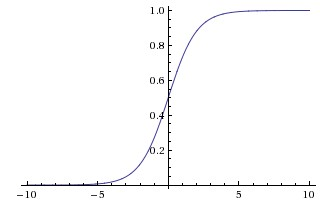
\includegraphics[width=4cm]{sigmoid}
    \caption{Sigmoid non-linearity squashes real numbers to range between [0,1]}
\end{figure}

%due to page break
\break
\break
\break

\textbf{\textit{tanh}} is a non-linear function which is similar in nature to the sigmoid.  The tanh uses real numbers with values ranging from [-1,1].  The tanh function has the same draw back as the sigmoid function with respect to saturation near the limits and since the tanh is not centered around zero, the function is preferred over the sigmoid function.  Since, the function in not zero centered only zero values are zero and thus the tanh function is less likely to have the same ill desired affect during the training of the network. 

\begin{center}
$tanH(\theta) = \frac{sinh(\theta)}{cosh(\theta)}$ = $\frac{e - e^-z}{e - e^-z}$
\end{center}
\begin{figure}[h] %[h] = place here
    \centering
    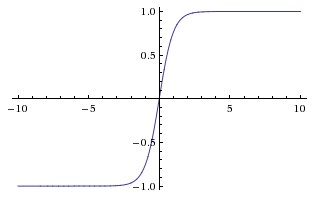
\includegraphics[width=4cm]{tanh}
    \caption{tanh non-linearity squashes real numbers to range between [-1,1]}
\end{figure}

\textbf{\textit{Rectified Linear Unit (ReLU)}} is a non-linear function shown in Fig. 7.  The ReLU has been show to operate a an accelerate rate compared to the sigmoid and tahn activation function.  However, the ReLU does have one major problem which is caused be large gradients recursively flowing back through the network.  These large gradients can sometimes cause the neuron to not fire causing loos of signal.  This effectively cause the network to not learn by not passing the signal through the neurons for all input-output data pairs.  Selecting a proper training rate can greatly reduce this frequency of this phenomena.

\begin{center}
$f(x) = max(0,x)$
\end{center}

\hfill\break
\begin{figure}[h]
    \centering
    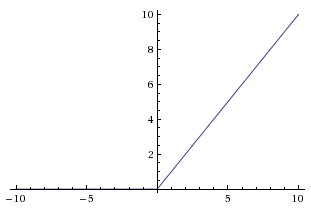
\includegraphics[width=4cm]{relu}
    \caption{Rectified Linear Unit (ReLU) activation function, which is zero when x < 0 and then linear with slope 1 when x > 0}
\end{figure}

\textbf{\textit{Leaky ReLU}} is a form of the ReLU and introduces a small slope which attempts to corrects the loss of firing on neuron or "dying neurons".  The Leaky ReLU introduces a small negative slope.  More studies are need here to determine if the slope has a positive impact as the results are not always conclusive.
\hfill\break
\begin{center}
$f(x) = 1(x<0)(\theta x) + 1(x >= 0)(x)$
\end{center}

\hfill\break
\begin{figure}[h]
    \centering
    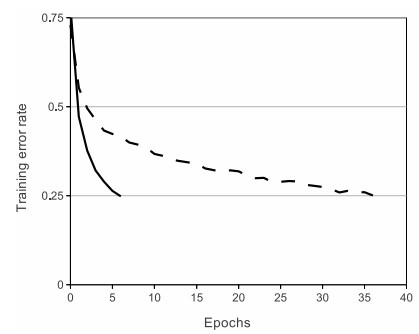
\includegraphics[width=4cm]{leakyrelu}
    \caption{A plot \cite{imageClassification} indicating the 6x improvement in convergence with the ReLU unit compared to the tanh unit.}
\end{figure}

%Added Merl 28-Sept-2017
\subsection{Gradient}
The gradient decent is the derivative of the squared error function with respect to the weights of the network.  The gradient decent is used to minimize the error function $f(x)$ by performing data manipulation on the on the weights $(w)$ that are placed on each connection.  The gradient descent is used in conjunction with backpropagation
\begin{figure}[h]
    \centering
    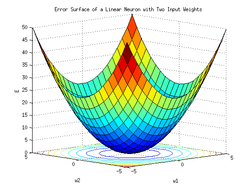
\includegraphics[width=4cm]{gradient}
    \caption{Gradient Decent}
\end{figure}

\subsection{Back-propagation}
Back-propagation is a methodology used in artificial neural networks to compute each node's or neuron's error contribution after the consumption of a single set of input signals.  Back-propagation is used in conjunction with supervised neural networks because back-propagation requires known, desired output signal for each set of input signals. This process uses an optimized algorithm to adjust the weights for each neuron after completing the learning process for that set of input signals.

Back-propagation is a generalization of the delta rule to multi-layered feed-forward networks, made possible by using the chain rule to iteratively compute a gradient cost for each layer. The back-propagation algorithm has been repeatedly rediscovered and is a special case of a more general technique called automatic differentiation in reverse accumulation mode. It is closely related to the Gauss–Newton algorithm.

Back-propagation is also sometimes referred to as deep learning, which is a term used to describe neural networks with more than one hidden layer.  It is also call backward propagation of error because the mean square error is calculated at the output neuron and then distributed back through each layers connections.

\begin{center}
\line(1,0){250}
\end{center}
\subsubsection{Problem Definition}
\begin{itemize}
    \item Dataset consisting of input-output pairs $(\vec{x_i},\vec{y_i})$, where $\vec{x_i}$ is the input and $\vec{y_i}$ is the desired output of the network on input $\vec{x_i}$.  The set of input-output pairs of size $N$ is denoted $X = {(\vec{x_i},\vec{y_i}), \dots,(\vec{x_N},\vec{y_N})}$.
    \item A feedforward neural network, as formally defined in the article concerning feedforward neural networks, whose parameters are collectively denoted $\theta$.  In backpropagation, the parameters of primary interest are $w_{ij}^k$, the weight between node $j$ in layer $l_k$ and node $i$ in layer $l_{k-1}$, the bias for node $i$ in layer $l_k$.  There are no connections between nodes in the same layer and layers are fully connected.
    \item An error function, $E(X, \theta)$, which defines the error between the desired output $\vec{y_i}$ and the calculated output $\hat{\vec{y_i}}$ of the neural network on input $\vec{x_i}$ for a set of input-output pairs $(\vec{x_i}, \vec{y_i}) \in X$ and a particular value of the parameters $\theta$.
\end{itemize}

Training a neural network with gradient descent requires the calculation of the gradient of the error function $E(X, \theta)$ with respect to the weights $w_{ij}^k$ and biases $b_i^k$. Then, according to the learning rate $\alpha$  each iteration of gradient descent updates the weights and biases (collectively denoted $\theta$ according to:
\begin{center}
$\theta^{t+1} = \theta^{t} - \alpha \frac{\partial E(X, \theta^{t})}{\partial \theta}$
\end{center}
where $\theta^{t}$ denotes the parameters of the neural network at iteration $t$ in gradient descent.

\begin{center}
\line(1,0){250}
\end{center}
\subsubsection{Neural Network forwardfeed General formulas}
\begin{itemize}
    \item $w_{ij}^k$: weight for node $j$ in layer $l_k$ for incoming node $i$ $b_i^k$ bias for node $i$ in layer $l_k$
    \item $a_i^k$: product sum plus bias for node $i$ in layer $l_k$
    \item $o_i^k$: output node for $i$ in layer $l_k$
    \item $r_k$: number of nodes in layer $l_k$
\end{itemize}

The mean squared error is the error function mainly in backpropagation.
\begin{center}
    $E(X, \theta) = \frac{1}{2N} \sum_{i=1}^N \left(\hat{y_i} - y_i\right)^2$
\end{center}
where $y$ is the target value for input-output pair $(\vec{x_i},y_i)$ and $\hat{y_i}$ is the computed output of the network on input $\vec{x_i}$. 
% More work could be done here other error functions can be used, but the mean squared error's historical association with backpropagation 

\begin{center}
\line(1,0){250}
\end{center}
\subsubsection{Backpropagation Algorithm}
\begin{itemize}
    \item Calculate the forward feed for each input-output pair $(\vec{x_d},y_d)$ and store the results $\hat{y_d},a_j^k$, and $o_j^k$ for each node $j$ in layer $k$ by proceeding from layer the input layer $0$, to layer $m$ , the output layer.
    \item Calculate the backwards feed for each input-output pair $(\vec{x_d},y_d)$ and store the results $(\frac{\partial E_d}{\partial w_{ij}^k})$ for each weight $w_{ij}^k$ connecting node $i$ in layer $k - 1$ to node $j$ in layer $k$ by proceeding from layer $m$, the output layer, to layer  the input layer.
    \begin{enumerate}
     \item Evaluate the error term for the final layer $\delta_1^k$ by using the second equation.
     \item Backpropagate the error terms for the hidden layers $\delta_j^k$ working backwards from the final hidden layer $k = m - 1$, by repeatedly using the third equation.
     \item Evaluate the partial derivatives of the individual error $E_d$ with respect to $w_{ij}^k$ by using the first equation.
    \end{enumerate}
    \item Combine the individual gradients for each input-output pair $(\frac{\partial E_d}{\partial w_{ij}^k})$ to get the total gradient $(\frac{\partial E(X, \theta)}{\partial w_{ij}^k})$ for the entire set of input-output pairs 
    $X = \{(\vec{x_1}, y_1), \dots, (\vec{x_N}, y_N) \}$ by using the fourth equation (a simple average of the individual gradients).
    \item Update the weights according to the learning rate $alpha$ and total gradient $(\frac{\partial E(X, \theta)}{\partial w_{ij}^k})$ by using the fifth equation (moving in the direction of the negative gradient).
\end{itemize}

%need proof here
\begin{center}
\line(1,0){250}
\end{center}
\subsubsection{Proof}

The XOR example described below will prove that the XOR gate can be solved using the Object Oriented Principals using the sigmoid function.

\hfill\break
The derivation of the sigmoid function is as follows and will show that Proof that $f(x) * (1 - f(x) = \frac{d}{dx} = \frac {e^{-x}}{(1 - e^{-x})^{2}}$
hold true.

\hfill\break
\begin{tabular}{ l }
     $f(x) = \frac{1}{1 - e^{-x}}$ \tabularnewline \\ 
     $\frac{d}{dx} = 1(1 - e^{-x})^{-1}$ \tabularnewline \\  
     $\frac{d}{dx} = -(1 - e^{-x})^{-2}$ \tabularnewline \\
     $\frac{d}{dx} = -(1 - e^{-x})^{-2} * (0 + e^{-x}\frac{d}{dx}(-x))$ \tabularnewline \\
     $\frac{d}{dx} = -(1 - e^{-x})^{-2} * (0 + e^{-x} * 1)$ \tabularnewline \\
     $\frac{d}{dx} = \frac {e^{-x}}{(1 - e^{-x})^{2}}$
\end{tabular}

\hfill\break
\begin{tabular}{ l }
    $\frac {e^{-x}}{(1 - e^{-x})^{2}} = f(x) * (1 - f(x))$ \tabularnewline \\ 
    $\frac{d}{dx}S(x) = \frac{e^{-x} + 1 - 1}{(1 + e^{-x})^{2}}$ \tabularnewline \\ 
    $\frac{d}{dx}S(x) = \frac{1 + e^{-x}}{(1 + e^{-x})^{2}} - \frac{1}{(1 - e^{-x})^{2}}$ \tabularnewline \\
    $\frac{d}{dx}S(x) = \frac{1}{1 + e^{-x}} - \frac{1}{(1 + e^{-x})^{2}}$ \tabularnewline \\
    $\frac{d}{dx}S(x) = \frac{1}{1 + e^{-x}} - \frac{1}{1 + e^{-x}} * \frac{1}{1 + e^{-x}}$ \tabularnewline \\
    $\frac{d}{dx}S(x) = \frac{1}{1 + e^{-x}} * [\frac{1}{1 + e^{-x}} - \frac{1}{1 + e^{-x}}]$
\end{tabular}
    
\break
\break
\break
For each neuron on each layer, the algorithm must compute the sum of all weighted connections from all incoming neurons.  So, for the first (top neuron in Fig 10), the algorithm must compute the sum of inputs pairs [1,1] with weights [.8, 2].  This must be done for each neuron, in each layer.  This may be computed $\sum_{j}^{l_k} w_{i}$.  \textit{Refer to Neural Network forwardfeed General formulas}

Hidden layer calculations
\begin{enumerate}
    \item $j_1$ 
    \begin{itemize}
        \item $i = 1, w_{ij}^k = .8$, yields $1 * .8 = .8$
        \item $i = 1, w_{ij}^k = .2$, yields $1 * .2 = .2$
        \item yields $.8 + .2 = 1$
    \end{itemize}
    \item $j_2$ 
    \begin{itemize}
        \item $i = 1, w_{ij}^k = .4$, yields $1 * .4 = .4$
        \item $i = 1, w_{ij}^k = .9$, yields $1 * .9 = .9$
        \item yields $.4 + .9 = 1.3$
    \end{itemize}
    \item $j_3$ 
    \begin{itemize}
        \item $i = 1, w_{ij}^k = .5$, yields $1 * .5 = .5$
        \item $i = 1, w_{ij}^k = .3$, yields $1 * .3 = .3$
        \item yields $.5 + .3 = .8$
    \end{itemize}
\end{enumerate}

Output Layer calculations are compute using the following derivation of the sigmoid function $f(x) * (1 - f(x)$

\begin{figure}[h]
    \centering
    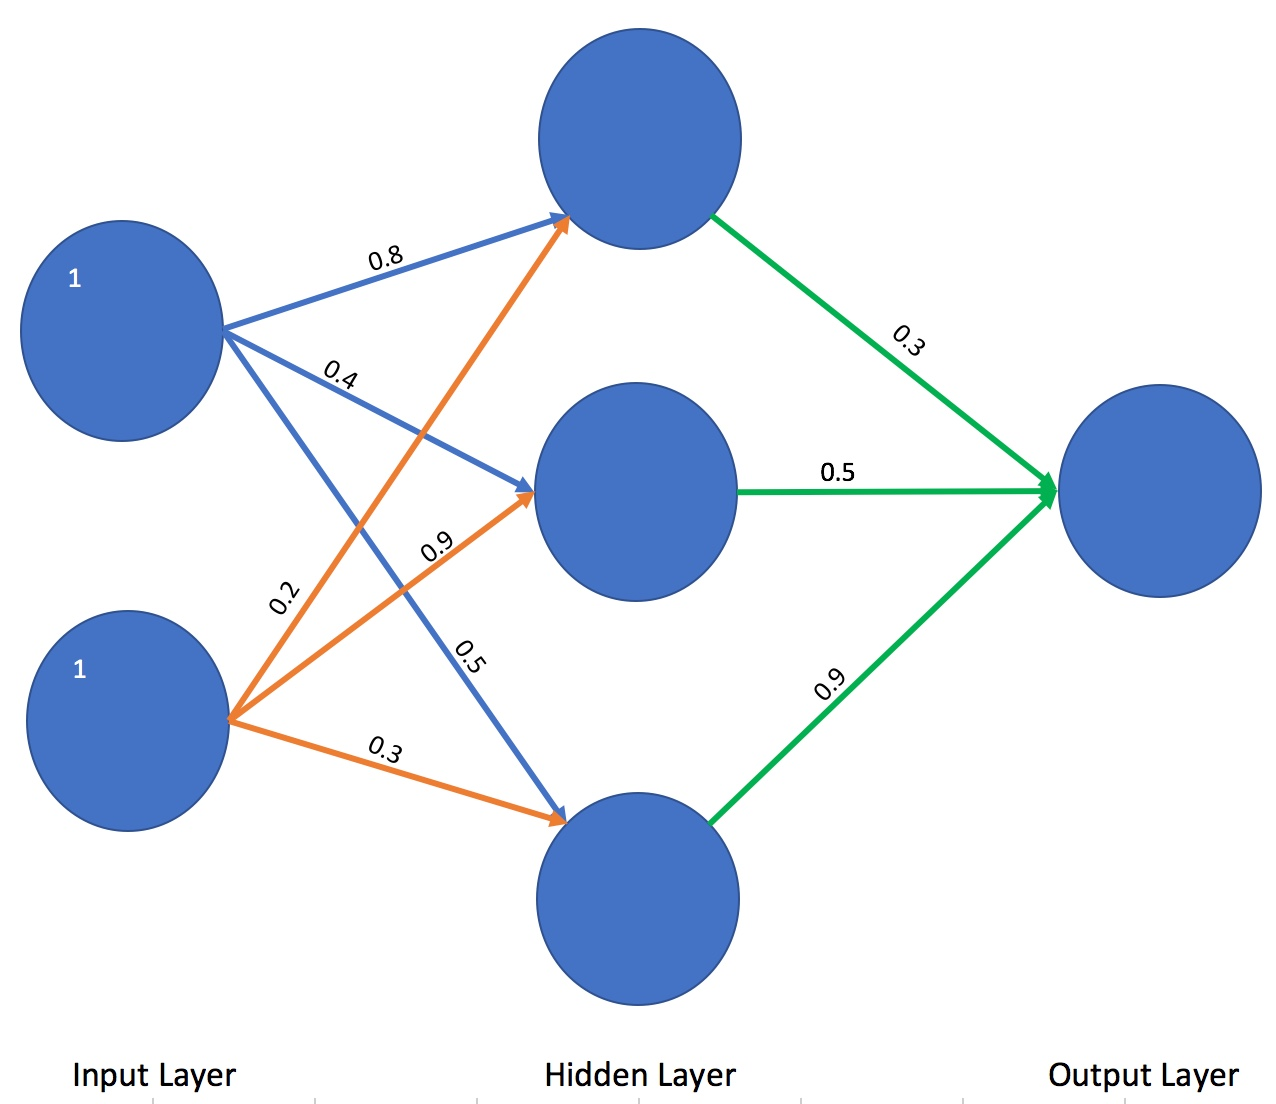
\includegraphics[width=8cm]{xor}
    \caption{XOR Neural Network with weighted connections, for input [1,1]}
\end{figure}




\section{Add Your Math, Algorithm here}

%Here is the conclusion
\section{Conclusion}

\section{APPENDIX}

Appendixes should appear before the acknowledgment.

\section{ACKNOWLEDGMENT}

Put sponsor acknowledgments in the unnumbered footnote on the first page.

% See below for IEEE bibliography 9/26/17 Jared
\bibliography{reference.bib}
\bibliographystyle{IEEEtran}

\end{document}
